\documentclass[10pt,landscape]{article}
\usepackage{multicol}
\usepackage{calc}
\usepackage{ifthen}
\usepackage[portrait]{geometry}
\usepackage{amsmath,amsthm,amsfonts,amssymb}
\usepackage{color,graphicx,overpic}
\usepackage{hyperref}
\usepackage{listings}
\usepackage{graphicx}




\pdfinfo{
  /Title (example.pdf)
  /Creator (TeX)
  /Producer (pdfTeX 1.40.0)
  /Author (Seamus)
  /Subject (Example)
  /Keywords (pdflatex, latex,pdftex,tex)}

% This sets page margins to .5 inch if using letter paper, and to 1cm
% if using A4 paper. (This probably isn't strictly necessary.)
% If using another size paper, use default 1cm margins.
\ifthenelse{\lengthtest { \paperwidth = 11in}}
    { \geometry{top=.5in,left=.5in,right=.5in,bottom=.5in} }
    {\ifthenelse{ \lengthtest{ \paperwidth = 297mm}}
        {\geometry{top=1cm,left=1cm,right=1cm,bottom=1cm} }
        {\geometry{top=1cm,left=1cm,right=1cm,bottom=1cm} }
    }

% Turn off header and footer
\pagestyle{empty}

% Redefine section commands to use less space
\makeatletter
\renewcommand{\section}{\@startsection{section}{1}{0mm}%
                                {-1ex plus -.5ex minus -.2ex}%
                                {0.5ex plus .2ex}%x
                                {\normalfont\large\bfseries}}
\renewcommand{\subsection}{\@startsection{subsection}{2}{0mm}%
                                {-1explus -.5ex minus -.2ex}%
                                {0.5ex plus .2ex}%
                                {\normalfont\normalsize\bfseries}}
\renewcommand{\subsubsection}{\@startsection{subsubsection}{3}{0mm}%
                                {-1ex plus -.5ex minus -.2ex}%
                                {1ex plus .2ex}%
                                {\normalfont\small\bfseries}}
\makeatother

% Define BibTeX command
\def\BibTeX{{\rm B\kern-.05em{\sc i\kern-.025em b}\kern-.08em
    T\kern-.1667em\lower.7ex\hbox{E}\kern-.125emX}}

% Don't print section numbers
\setcounter{secnumdepth}{0}


\setlength{\parindent}{0pt}
\setlength{\parskip}{0pt plus 0.5ex}

%My Environments
\newtheorem{example}[section]{Example}
% -----------------------------------------------------------------------

\begin{document}
\raggedright
\footnotesize
\begin{multicols}{2}


% multicol parameters
% These lengths are set only within the two main columns
%\setlength{\columnseprule}{0.25pt}
\setlength{\premulticols}{1pt}
\setlength{\postmulticols}{1pt}
\setlength{\multicolsep}{1pt}
\setlength{\columnsep}{2pt}

\begin{center}
     \Large{\underline{CS142-Cheatsheet}} \\
\end{center}

\section*{html and css}
\begin{itemize}
\item Hello World
\begin{verbatim}
<?xml version="1.0" encoding="utf-8"?>
<!DOCTYPE html PUBLIC "-//W3C//DTD XHTML 1.0 Strict//EN"
    "http://www.w3.org/TR/xhtml1/DTD/xhtml1-strict.dtd">
<html xmlns="http://www.w3.org/1999/xhtml" 
xml:lang="en" lang="en">
  <head>
    <title>Hello World</title>
  </head>
  <body>
    <p>Hello world!</p>
  </body>
</html>
\end{verbatim}
\item Start tag contain attributes 
\begin{verbatim}
<img src="face.jpg">
<input type="text" value="94301" name="zip">
<div class="header">
\end{verbatim}
\item Include as a link:
\begin{verbatim}
<link rel="stylesheet" type="text/css" href="myStyles.css" />
\end{verbatim}
\item Include in the body
\begin{verbatim}
<style type="text/css">
    body {
        font-family: Tahoma, Arial, sans-serif;
        ...
    }
</style>
\end{verbatim}
\end{itemize}
\section*{URLs}
\begin{itemize}
\item Multi-level escaping: \verb|<a href="/a/b/c?name=C%26H%20Sugar&year=2006">|

\end{itemize}
\section*{Ruby Laguage}
\begin{itemize}
\item \textbf{Scope} local: \verb|foo|, global: \verb|$foo|; instance variable: \verb|@foo|; class variable: \verb|@@foo|;
\item single quote : \verb|%q<Nesting works: <b>Hello</b>>|
\item hashes: \verb|order = {"item" => "Corn Flakes", "weight" => 18}| or  \verb|order = {item: "Corn Flakes", weight: 18}|
\item \textbf{Append to a list} \verb|@primes << candidate|
\item Module Example 
\begin{verbatim}
class MyClass
  include Enumerable
  ...
  def each
    ...
  end
  def <=>
    ...
  end
end
\end{verbatim}
\item\textbf{ Many Arguments:}
\begin{verbatim}
def max(first, *rest)
  result= first
  for x in rest do
    if (x > result) then
      result= x
    end
  end
  return result
end
\end{verbatim}

\item \textbf{Iterators and Resuable}
\begin{verbatim}
 def sum_odd(count)
    sum = 0
    odd_numbers(count) do |i|
        sum += i
    end
    return sum
end

def odd_numbers(count)
    number = 1
    while count > 0 do
        yield(number)
        number += 2
        count -= 1
    end
end
\end{verbatim}
\item \textbf{Class}
\begin{verbatim}
class Point
  def initialize(x, y)
    @x = x
    @y = y
  end
  
  def x
    @x
  end
  
  def x=(value)
    @x = value
  end
end

\end{verbatim}
\end{itemize}
\section*{Rails}
\begin{itemize}
\item \textbf{Rails Structure:}
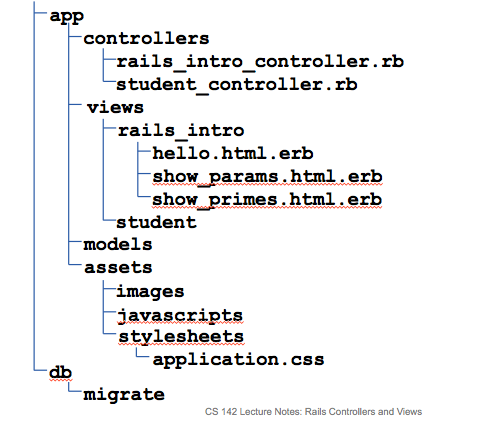
\includegraphics[width = \linewidth]{structure.png}
\item \textbf{Partial Page:} 
\begin{verbatim}
<%= render(:partial => "shared/foo",
:locals => {:x => 24, :y =>36}) %>
\end{verbatim}
 \item \textbf{Helper Functions} 
 \begin{verbatim}
<%= link_to(@name, {:action => :user_info, :id => @user_id}) %>
<%= image_tag "icon.jpg" %>
<%= stylesheet_link_tag "main" %>
<%= javascript_include_tag "file1", "file2" %>
 \end{verbatim}
\end{itemize}
\section*{SQL}
\begin{itemize}
\item \textbf{Create a table}
\begin{verbatim}
CREATE TABLE students (
    id INT AUTO_INCREMENT,
    name VARCHAR(30),
    birth DATE,
    gpa FLOAT,
    grad INT,
    PRIMARY KEY(id));
\end{verbatim}
\item \textbf{Add Rows}
\begin{verbatim}
INSERT INTO students(name, birth, gpa, grad)
     VALUES ('Anderson', '1987-10-22', 3.9, 2009);

\end{verbatim}
\item \textbf{Delete and Drop Tab}
\begin{verbatim}
DELETE FROM students WHERE name='Anderson';
DROP TABLE students;
\end{verbatim}
\item \textbf{Some Select Update Example}
\begin{verbatim}
SELECT gpa, name, grad
    FROM students
    WHERE gpa > 3.0
    ORDER BY gpa DESC;
 UPDATE students
    SET gpa = 2.6, grad = 2013
    WHERE id = 2;
\end{verbatim}
\item \textbf{Joins}
\begin{verbatim}
SELECT s.name, s.gpa
    FROM students s, advisors p
    WHERE s.advisor_id = p.id AND p.name = 'Fujimura';
\end{verbatim}
\item \textbf{Mega Example}
\begin{verbatim}
SELECT s.name, c.quarter
    FROM students s, courses c, courses_students cs
    WHERE c.id = cs.course_id AND s.id = cs.student_id
    AND c.number = 'ART101';
\end{verbatim}
\end{itemize}
\section*{Active Record}
\begin{itemize}
\item \textbf{Basic Operations}
\begin{verbatim}
student = Student.find(187)
student = Student.find_by_name("Hernandez")
smarties = Student.find(:all,
        :conditions => "gpa >= 3.0")
smarties = Student.find(:all, :limit => 10,
        :order => "gpa DESC")
Student.find(187).destroy()
\end{verbatim}
\item \textbf{One to Many, Many to Many  }
\begin{verbatim}
class Student < ActiveRecord::Base
    has_and_belongs_to_many :courses
end
class Course < ActiveRecord::Base
    has_and_belongs_to_many :students
end
_____________________________________
class Student < ActiveRecord::Base
    has_and_belongs_to_many :courses
end
class Course < ActiveRecord::Base
    has_and_belongs_to_many :students
end
\end{verbatim}
\item \textbf{Create Table}
\begin{verbatim}
class CreateStudents < ActiveRecord::Migration
    def change
        create_table :students do |t|
            t.column :name,        :string
            t.column :birth,       :date
            t.column :gpa,         :float
            t.column :grad,        :integer
        end
    end
end
\end{verbatim}
\item \textbf{Add Columns}
\begin{verbatim}
class AddAdvisor < ActiveRecord::Migration
    def change
        add_column :students, :advisor_id, :integer
    end
end
\end{verbatim}
\end{itemize}
\section*{http and https}
\begin{verbatim}
GET /index.html HTTP/1.1
Host: www.example.com
User-Agent: Mozilla/5.0
Accept: text/xml,application/xml,application/xhtml+xml,text/html*/*
Accept-Language: en-us
Accept-Charset: ISO-8859-1,utf-8
Connection: keep-alive
<blank line>
_______________
HTTP/1.1 200 OK
Date: Thu, 24 Jul 2008 17:36:27 GMT
Server: Apache-Coyote/1.1
Content-Type: text/html;charset=UTF-8
Content-Length: 1846

<?xml version="1.0" encoding="utf-8"?>
<!DOCTYPE html PUBLIC ... >
<html ... >
...
</html>
\end{verbatim}
\section*{Cookies Sessions}
\begin{verbatim}
Set-Cookie: session=0x4137fd6a; Expires=Wed, 09 Jun 2012 10:18:14 GMT
Cookie: session=0x4137fd6a
\end{verbatim}
\section*{Forms}
\begin{itemize}
\item \textbf{Form html}
\begin{verbatim}
<form action="/product/update" method="post">
  Product: <input type="text" name="product"/><br />
  Price: <input type="text" name="price" value="49.95"/><br />
  <input type="submit" value="Submit"/>
</form>
\end{verbatim}
\item \textbf{Form Tag}
\begin{verbatim}
<%= form_for(@student, method: :post,
    url: {action: :update, id: @student.id}) do |form| %>
  <%= form.text_field(:name) %>
  <%= form.text_field(:birth) %>
  <%= form.text_field(:gpa) %>
  <%= form.text_field(:grad) %>
  <%= form.submit "Modify Student" %>
<% end %>
\end{verbatim}
\item \textbf{Update Backend}
\begin{verbatim}
def update
  @student = Student.find(params[:id])
  if @student.update(student_params(params[:student])) then
    redirect_to(:action => :show)
  else
    render(:action => :edit)
  end
end

private
def student_params(params)
  return params.permit(:name, :birth, :gpa, :grad)
end
def create
  @student = Student.new(student_params(params[:student]))
  if @student.save then
    redirect_to(:action => :show)
  else
    render(:action => :edit)
  end
end
\end{verbatim}
\item \textbf{Validation}
\begin{verbatim}
class Student < ActiveRecord::Base
  validates_format_of :birth, :with => /\d\d\d\d-\d\d-\d\d/,
      :message => "must have format YYYY-MM-DD"
  def validate_gpa
    if (gpa < 0) || (gpa > 4.0) then
      errors.add(:gpa, "must be between 0.0 and 4.0")
    end
  end
  validate :validate_gpa
end
\end{verbatim}
\item \textbf{Form Errors}
\begin{verbatim}
<% @student.errors.full_messages.each do |msg| %>
  <p><%= msg %></p>
<% end %>
\end{verbatim}
\item \textbf{Files Upload}
\begin{verbatim}
<form method="POST" enctype="multipart/form-data">
form.file_field :photo
\end{verbatim}
\end{itemize}
% You can even have references
\rule{0.3\linewidth}{0.25pt}
\scriptsize
\bibliographystyle{abstract}
\bibliography{refFile}
\end{multicols}
\end{document}